%% LyX 2.2.2 created this file.  For more info, see http://www.lyx.org/.
%% Do not edit unless you really know what you are doing.
\documentclass[spanish]{article}
\usepackage[T1]{fontenc}
\usepackage{geometry}
\geometry{verbose,tmargin=2.25cm,bmargin=2cm,lmargin=2.25cm,rmargin=2cm}
\usepackage{float}
\usepackage{graphicx}

\makeatletter
%%%%%%%%%%%%%%%%%%%%%%%%%%%%%% User specified LaTeX commands.
\usepackage{fancyhdr}
\usepackage{lscape}
\pagestyle{fancy}
\lhead{An\'alisis de Se\~nales y Sistemas Digitales 22.05}
\chead{TPL1}
\rhead{ITBA}
\renewcommand{\headrulewidth}{1pt}
\renewcommand{\footrulewidth}{1pt}

\makeatother

\usepackage{babel}
\addto\shorthandsspanish{\spanishdeactivate{~<>}}

\begin{document}

\section{Implementaci\'{o}n en PCB - Consideraciones}

Dado que el sistema en su conjunto consiste de una parte anal\'{o}gica
y otra digital, es necesario tener en cuenta ciertas cuestiones al
momento de realizar la implementaci\'{o}n en PCB.

\subsection{Flancos digitales - Clocks}

Los osciladores que proveen las se\~{n}ales cuadradas de control para
la llave anal\'{o}gica y el sample \& hold exigen corriente al circuito
en los flancos, lo cual provoca una disminuci\'{o}n en la tensi\'{o}n
de alimentaci\'{o}n durante un breve lapso de tiempo, resultando agresivo
para el circuito anal\'{o}gico ya que \'{e}ste se encuentra conectado
a la misma l\'{\i}nea de alimentaci\'{o}n. Esto puede producir distorsiones
en las se\~{n}ales anal\'{o}gicas resultantes.

\begin{figure}[H]
\begin{centering}
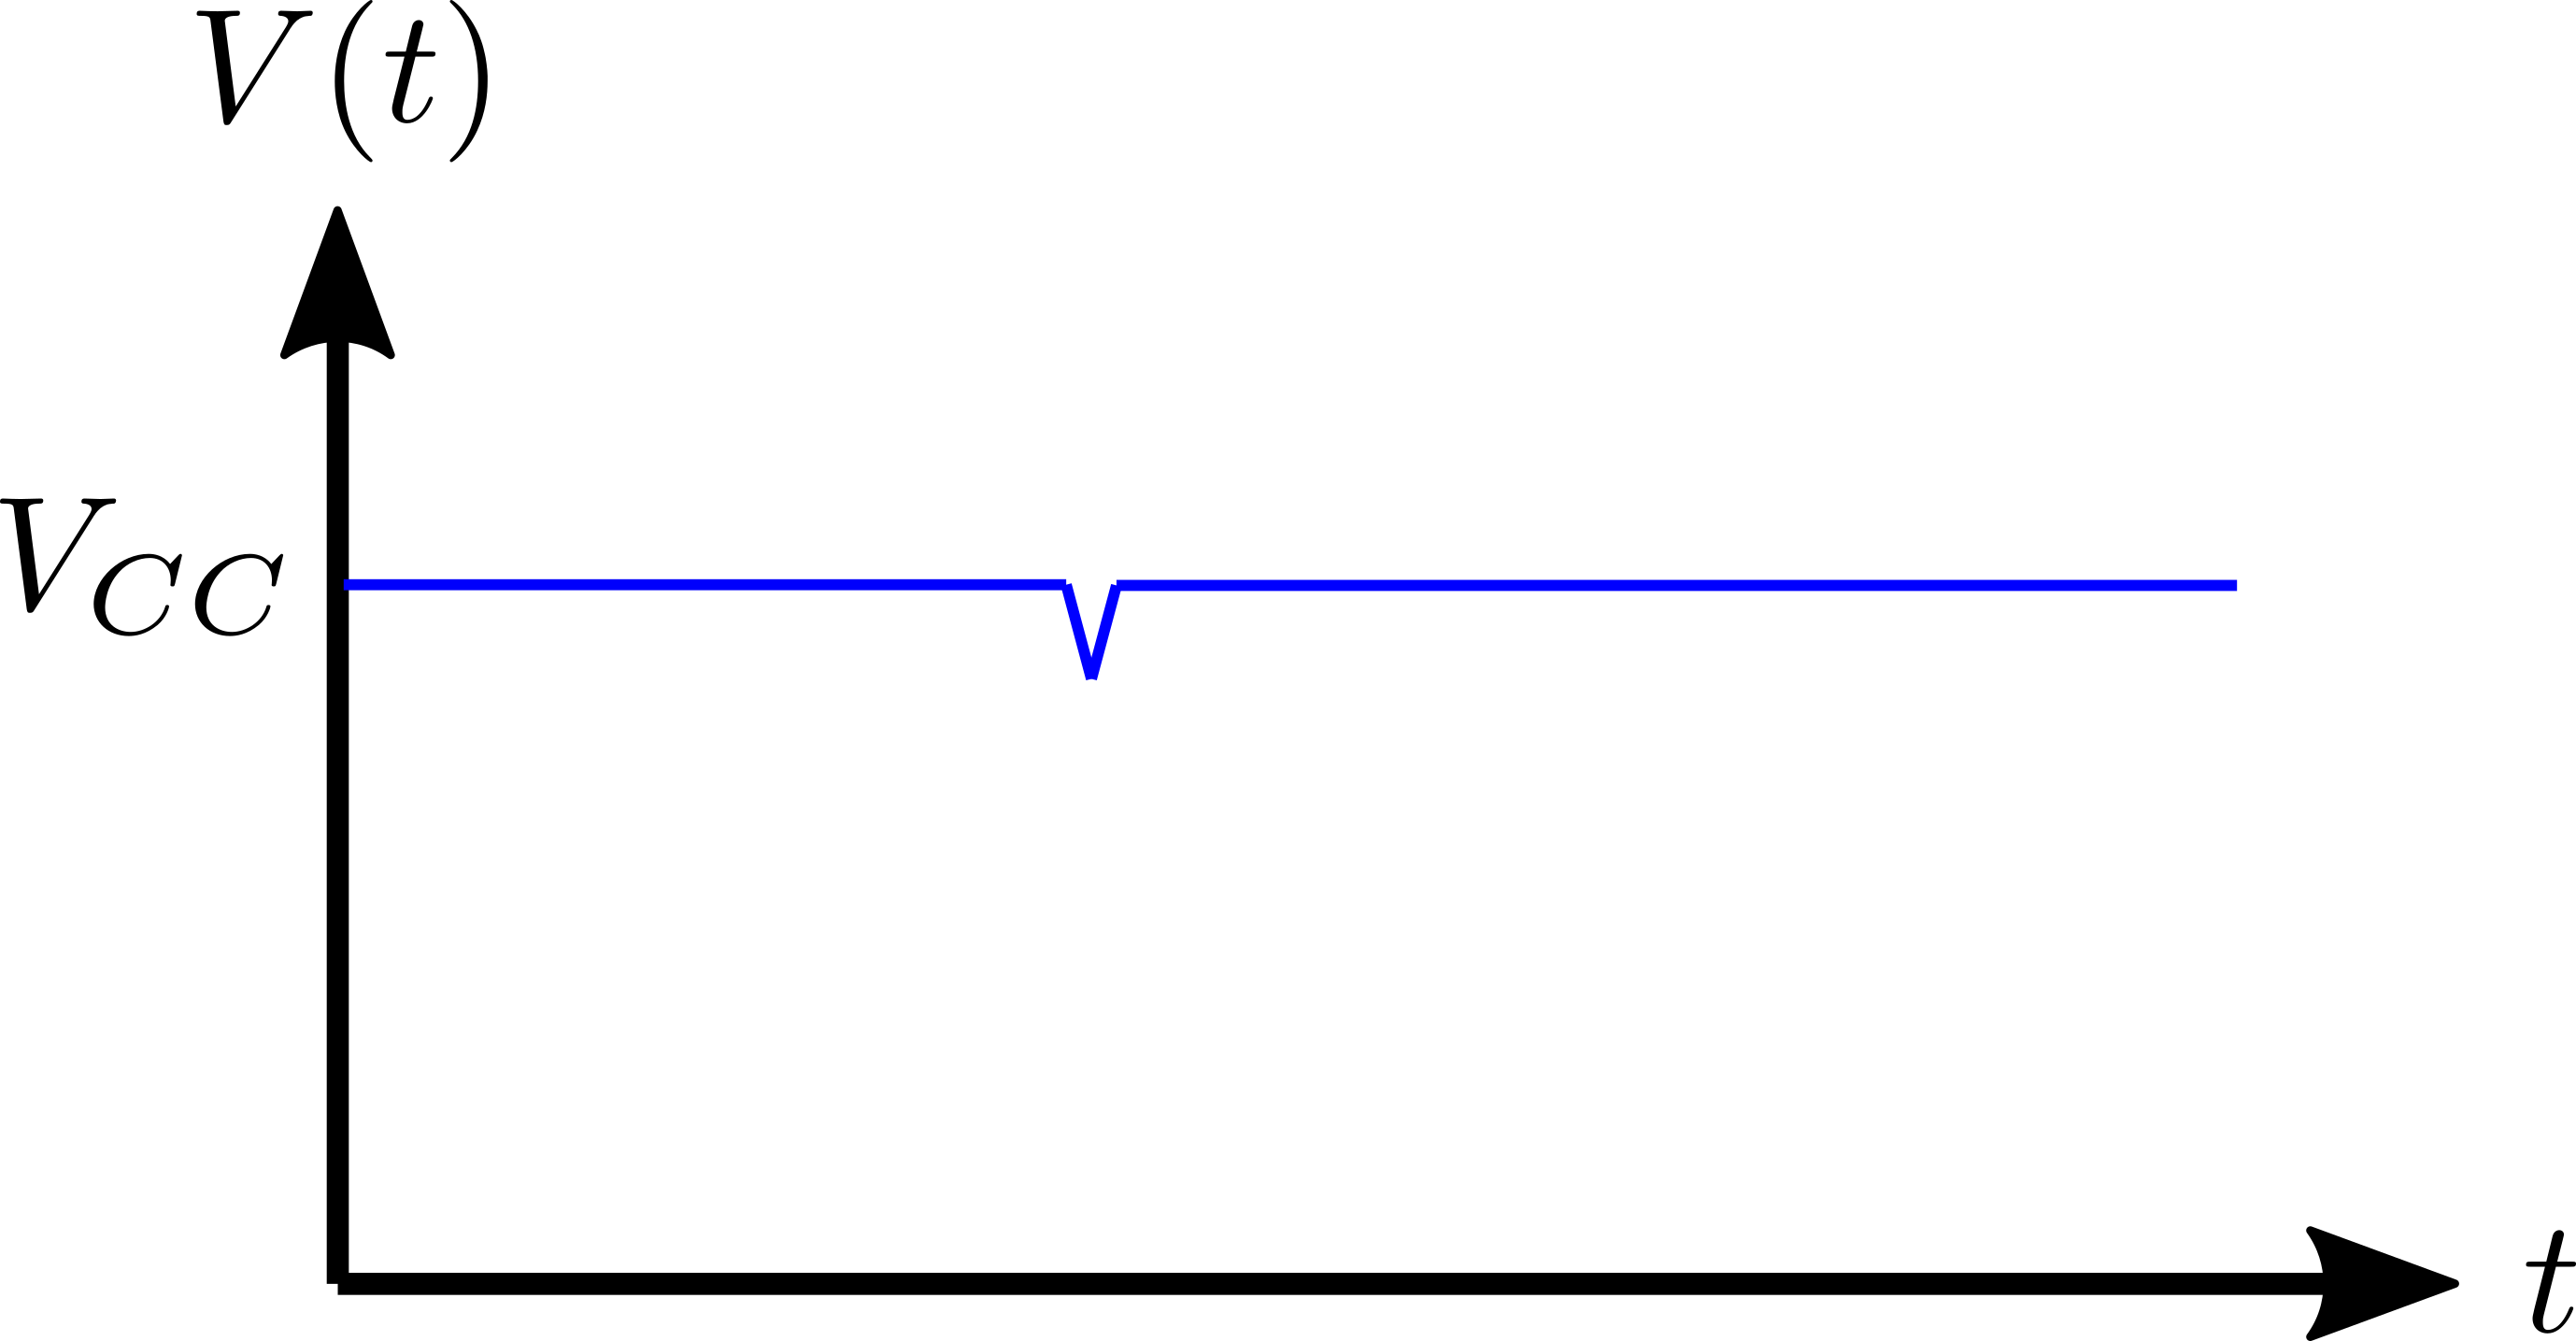
\includegraphics[scale=0.5]{Dibujos/Alimentacion}
\par\end{centering}
\caption{Alimentaci\'{o}n afectada por picos de corriente del circuito digital}

\end{figure}

El fen\'{o}meno en cuesti\'{o}n no es posible de eliminar en su totalidad,
pero si disminuirlo. Para ello se colocan capacitores de desacople
lo m\'{a}s cerca posible de los pines de alimentaci\'{o}n de los circuitos
integrados, de manera tal que puedan proveer r\'{a}pidamente una corriente
alta durante lapsos de tiempo breves, principalmente en los flancos
de las se\~{n}ales cuadradas. Se utilizaron capacitores multicapa
dado que pueden responder r\'{a}pidamente frente a estas situaciones.

Para proveer corrientes altas por per\'{\i}odos m\'{a}s largos, se
colocaron capacitores electrol\'{\i}ticos de $330uF$ creca del conector
de alimentaci\'{o}n de la placa, tanto en $+VCC$ como en $-VCC$.

\subsection{Divisi\'{o}n de circuitos}

Dado que las se\~{n}ales de clock poseen componentes de alta frecuencia,
si pasan cerca junto con las pistas que llevan se\~{n}ales anal\'{o}gicas
puede darse inducci\'{o}n entre ambas pistas, produciendo distorsi\'{o}n
sobre la se\~{n}al anal\'{o}gica. Para evitar esto, se separ\'{o}
por un lado a los circuitos osciladores en la parte digital, y a los
filtros e integrados de llave anal\'{o}gica y sample and hold por
otro, en zonas bien definidas como se muestra a continuaci\'{o}n.

\begin{figure}[H]
\begin{centering}
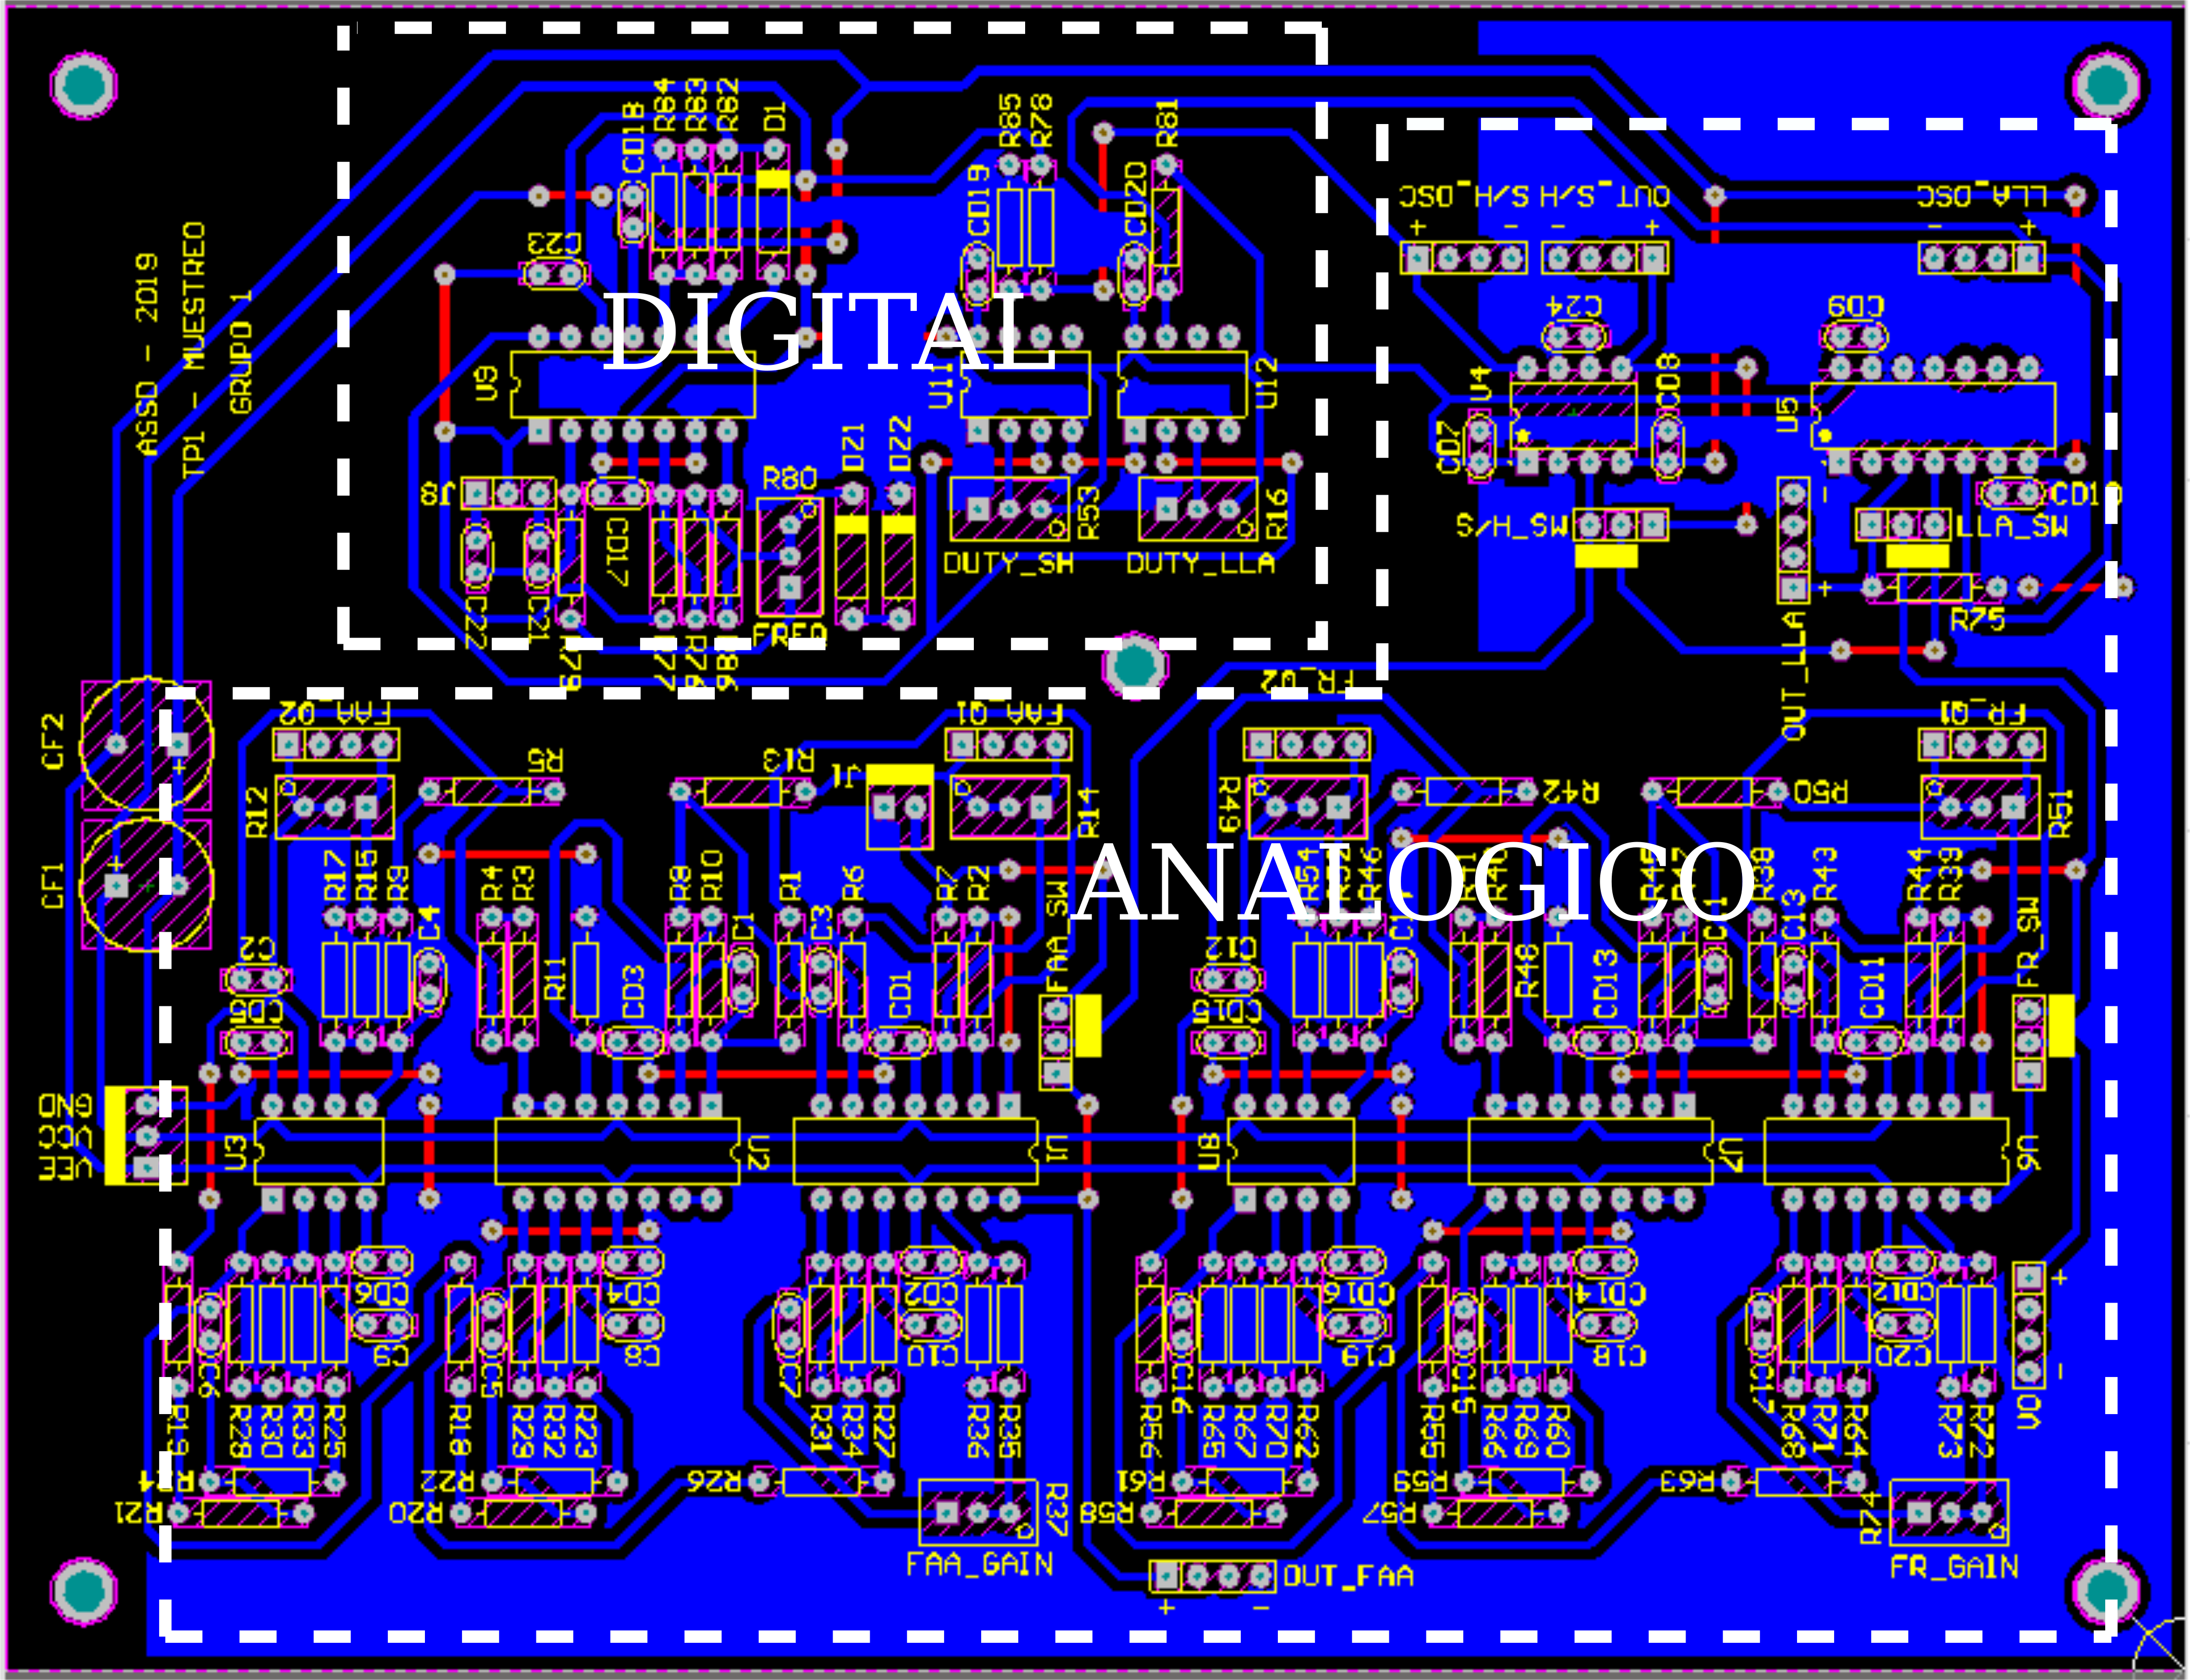
\includegraphics[scale=0.55]{Dibujos/ZonasMarcadas}
\par\end{centering}
\caption{Dise\~{n}o del PCB - Zonas}

\end{figure}

Para terminar de definir la divisi\'{o}n entre ambos circuitos, se
debe tener en cuenta que la corriente retorna por GND tambi\'{e}n.
Por lo tanto, se llev\'{o} una pista de GND por la circuiter\'{\i}a
anal\'{o}gica del sistema, sin pasar por la digital, y viceversa,
uniendo ambas en un solo punto, siendo \'{e}ste el pin de GND del
conector de alimentaci\'{o}n del PCB. De esta forma, se logra separar
ambas masas.

\subsection{Otras consideraciones pr\'{a}cticas}
\begin{itemize}
\item Para el dise\~{n}o de los filtros, sabiendo que se utilizan los mismo
integrados, se llev\'{o} la alimentaci\'{o}n por debajo de los mismos
en linea recta directamente hacia el conector de alimentaci\'{o}n,
sin pasar por medio del circuito. Esto resulta pr\'{a}ctico dada la
posici\'{o}n de los integrados.
\item Se a\~{n}adieron pines de medici\'{o}n a la salida de las diferentes
etapas (lo m\'{a}s cerca posible de ellas), y jumpers para poder anular
o utilizar cualquiera de las etapas.
\item En las cuatro esquinas se colocaron tamecos para el soporte de la
placa, mas un tameco adicional en el centro, en una zona donde confluyen
4 presets. Esto es una medida de seguridad, ya que para calibrar los
presets se debe ejercer una cierta presi\'{o}n. Si no se tiene cuidado
puede doblarse el PCB, donde en el peor caso si se realiza reiteradas
veces pueden cortarse algunas pistas, debido a que la placa es de
fabricaci\'{o}n casera en pertinax, el cual es un material m\'{a}s
flexible que la fibra de vidrio.
\end{itemize}
El tama\~{n}o final resultante del PCB es de aproximadamente 14cm
x 18cm.

\begin{figure}[H]
\begin{centering}
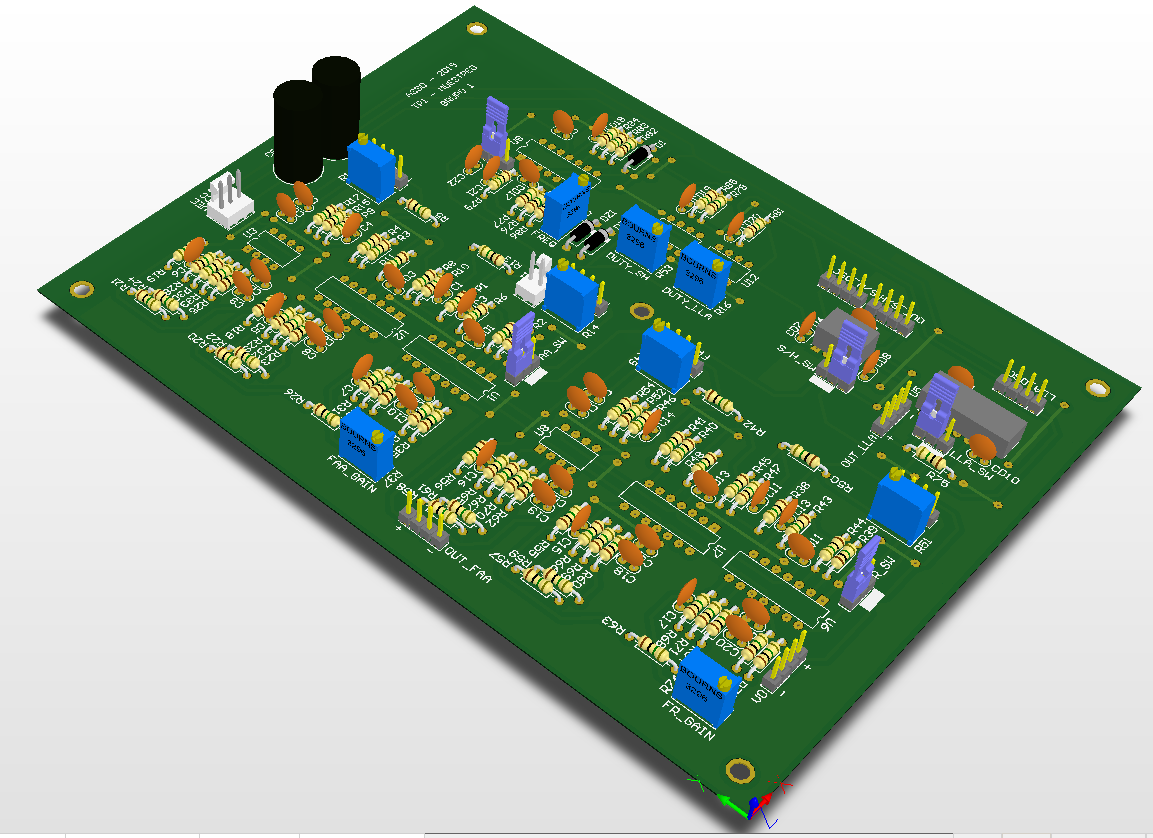
\includegraphics[scale=0.6]{Dibujos/modelo3D}
\par\end{centering}
\caption{Dise\~{n}o de PCB - Modelo 3D}

\end{figure}

\end{document}
